\documentclass[svgnames,t]{beamer}
\usepackage[english]{babel}
\usepackage{fontspec,mathabx,etoolbox,listings,tikz,multicol}

\setsansfont{Yanone Kaffeesatz}[
    UprightFont     = *-Regular ,
    BoldFont        = *-Bold ,
    BoldItalicFont  = *-Bold ,
    BoldSlantedFont = *-Bold ,
    ItalicFont      = *-Light ,
    SlantedFont     = *-Light ,
    SmallCapsFont   = *-Thin
]

%\setmonofont{Latin Modern Mono Prop}

\usetikzlibrary{
    overlay-beamer-styles,
    calc,
    positioning,
    decorations.pathreplacing,
    backgrounds, shadings,
    shapes
}

\tikzset{
    %Displaying keys
    onslide/.code args={<#1>#2}{\only<#1>{\pgfkeysalso{#2}}}, % \pgfkeysalso doesn't change the path
    scope on/.style={
        every node/.append style={visible on=#1},
        every path/.append style={visible on=#1}
    },
    %Path ending shapes
    to/.style={->,>=stealth},
    from/.style={<-,>=stealth},
    fromto/.style={<->,>=stealth},
    shorter/.style 2 args={shorten <= #1, shorten >= #2},
    %Hexagons
    hexagon/.style n args={3}{double arrow, double arrow head extend=0cm, inner sep=3pt, draw=#1, fill=#2, text=#3, thick},
    hexagon/.default={black}{gray!20}{black},
    hexagonOne/.style={hexagon={#1}{#1!30}{#1}},
    hexagonTwo/.style 2 args={hexagon={#1}{#1!#2}{#1}},
    hexagonThree/.style n args={3}{hexagon={#1}{#1!#2}{#3}},
    hexagonShade/.style n args={3}{double arrow, double arrow head extend=0cm, inner sep=3pt, thick, draw=#1, left color=#2, right color=#3},
    %General text element
    Shape/.style n args={3}{draw=#1, fill=#2, text=#3},
    genShape/.style 2 args={#1, inner sep=3pt, draw=#2, fill=#2!20, text=#2, thick},
    halo/.style={preaction={draw, #1, line width=7, -}},
}
\usepackage{listings}
\def\transpPerc{100}
%listings set
\lstdefinestyle{MyBash}{
% backgroundcolor=\color{white},    % choose the background color; you must add \usepackage{color} or \usepackage{xcolor}
breakatwhitespace=false,            % sets if automatic breaks should only happen at whitespace
breaklines=true,                    % sets automatic line breaking
captionpos=b,                       % sets the caption-position to bottom
deletekeywords={...},               % if you want to delete keywords from the given language
escapeinside={@|}{|@},                % if you want to add LaTeX within your code
extendedchars=true,                 % lets you use non-ASCII characters; for 8-bits encodings only,
                                    % does not work with UTF-8
frame=none  ,                       % adds a frame around the code
numbers=none,                       % where to put the line-numbers; possible values are (none, left, right)
numbersep=5pt,                      % how far the line-numbers are from the code
numberstyle=\tiny\color{black},     % the style that is used for the line-numbers
rulecolor=\color{black},            % if not set, the frame-color may be changed on line-breaks within not-black text
                                    % (e.g. comments (green here))
showspaces=false,                   % show spaces everywhere adding particular underscores; it overrides 'showstringspaces'
showstringspaces=false,             % underline spaces within strings only
showtabs=false,                     % show tabs within strings adding particular underscores
stepnumber=2,                       % the step between two line-numbers. If it's 1, each line will be numbered
stringstyle=\color{OliveGreen},     % string literal style
tabsize=2,                          % sets default tabsize to 2 spaces
title=\lstname,                     % show the filename of files included with \lstinputlisting; also try caption instead of title
%
%Base style for this presentation 
keepspaces=true,                    % keeps spaces in text, useful for keeping indentation of code
                                    % (possibly needs columns=flexible)
keywordstyle=\color{Cyan},          % keyword style
language=C++,
basicstyle=\ttfamily\scriptsize\color{black},
keywordstyle=\color{OliveGreen},
stringstyle=\color{Magenta},
commentstyle=\color{red},
moredelim=[is][\color{ForestGreen}]{|+}{+|},
literate=% literate={<replace>}{<replacement text>}{<width>}
  {\#define}{{{\color{CarnationPink}\#define}}}{6}
  {\#include}{{{\color{CarnationPink}\#include}}}{7},
morekeywords={},
emph=[1]{},
emphstyle=[1]{\color{NavyBlue}}, %Functions
emph=[2]{},
emphstyle=[2]{\color{Orange}}, %Variables
emph=[3]{if, else, elif, fi, while, for, case, do, esac, done},
emphstyle=[3]{\color{violet}}, %Loops, if, etc.
emph=[4]{return, exit},
emphstyle=[4]{\color{ProcessBlue}}, %Logical keywords
emph=[6]{PATH, SHELL},
emphstyle=[6]{\color{Gray}}, %Environment variables
}

\lstnewenvironment{Bash}[1][]
    {\lstset{style=MyBash, belowskip=-7mm, aboveskip=0pt,#1}}
    {}

\def\bash{\lstinline[style=MyBash, basicstyle=\ttfamily\color{black}]}


\makeatletter
\newenvironment{CenteredBox}{% 
\begin{Sbox}}{% Save the content in a box
\end{Sbox}\centerline{\parbox{\wd\@Sbox}{\TheSbox}}}% And output it centered
\makeatother


\newcommand<>{\tc}[2]{\textcolor#3{#1}{#2}}
\newcommand{\tikzmark}[1]{\tikz[overlay,remember picture, baseline=-0.5ex] \node at (0,0) (#1) {};}
\newcommand{\URLsymbol}[2][white]{%
    \begin{tikzpicture}[every path/.style={line width=3, rounded corners, #2}]
        \pgfmathsetmacro{\longSide}{0.9}
        \pgfmathsetmacro{\shortSide}{0.3}
        \draw[rotate=45, xshift=0.5*\longSide cm]       (0,0) rectangle (\longSide, \shortSide);
        \draw[rotate=45, halo=#1, #2!50]                   (0,0) rectangle (\longSide, \shortSide);
        \draw[rotate=45, halo=#1, xshift=0.5*\longSide cm] (0, 0.5*\shortSide) -- (0,0) -- (\longSide, 0) -- (\longSide, 0.5*\shortSide);
    \end{tikzpicture}
}
\NewDocumentCommand{\URL}{ O{black} m m O{BGLIGHT} }%
{%
    \raisebox{-0.4ex}{\resizebox{!}{2ex}{\URLsymbol[#4]{#1}}}{\href{#2}{\textcolor{#1}{#3}}}
}

\NewDocumentCommand{\addSection}{ m O{} m m }%
{%
    \setbeamertemplate{section page}[Iceland][#2]{#3}{#4}
    \section{#1}
}

\makeatletter
\newcommand*\keystroke[1]
{%
    \begin{tikzpicture}[baseline=($(key.base)!0.8!(key.south)$), very thin]%
        \pgfmathsetlengthmacro{\textHeight}{0.9*\f@size}
        \pgfmathsetlengthmacro{\textHeightPlus}{1.25*\textHeight}
        \pgfmathsetlengthmacro{\roundedSmall}{0.2}
        \pgfmathsetlengthmacro{\roundedLarge}{0.4}
        \pgfmathsetlengthmacro{\dl}{0.5\pgflinewidth}
        \node[font=\sffamily, inner xsep=2pt, inner ysep=1pt] (text) {\scalebox{1.2}[0.75]{\textsmaller[2]{#1\strut}}};
        \node[rounded corners=\roundedLarge, minimum size=\textHeight, anchor=north west] (key) at (text.north west){};
        \node[rounded corners=\roundedSmall, minimum size=\textHeightPlus] (frame) at ($(key.center)!0.05!(key.south)$){};
        \path coordinate (keyNW) at ($(key.north west)+(\roundedLarge,-\dl)$)
              coordinate (keyNE) at ($(key.north east)-(\roundedLarge,+\dl)$)
              coordinate (keyEN) at ($(key.north east)-(-\dl,\roundedLarge)$)
              coordinate (keyES) at ($(key.south east)+(+\dl,\roundedLarge)$)
              coordinate (keySE) at ($(key.south east)-(\roundedLarge,+\dl)$)
              coordinate (keySW) at ($(key.south west)+(\roundedLarge,-\dl)$)
              coordinate (keyWS) at ($(key.south west)+(+\dl,\roundedLarge)$)
              coordinate (keyWN) at ($(key.north west)-(-\dl,\roundedLarge)$)
              coordinate (frameNW) at ($(frame.north west)+(\roundedSmall,-\dl)$)
              coordinate (frameNE) at ($(frame.north east)-(\roundedSmall,+\dl)$)
              coordinate (frameEN) at ($(frame.north east)-(+\dl,\roundedSmall)$)
              coordinate (frameES) at ($(frame.south east)+(-\dl,\roundedSmall)$)
              coordinate (frameSE) at ($(frame.south east)-(\roundedSmall,-\dl)$)
              coordinate (frameSW) at ($(frame.south west)+(\roundedSmall,+\dl)$)
              coordinate (frameWS) at ($(frame.south west)+(+\dl,\roundedSmall)$)
              coordinate (frameWN) at ($(frame.north west)-(-\dl,\roundedSmall)$);
        \foreach \n in {NW,NE,EN,ES,SE,SW,WS,WN}{
            \draw[line cap=round, ultra thin] (key\n) -- (frame\n);
        }
        \begin{scope}[on background layer]
            \node[draw, rounded corners=\roundedSmall, minimum size=\textHeightPlus, fill=fg] at ($(key.center)!0.05!(key.south)$){};
            \node[draw, rounded corners=\roundedLarge, lower right=gray!20, lower left=gray!50, upper right=gray!50, upper left=gray!80, minimum size=\textHeight, anchor=north west] at (text.north west){};
            \fill [gray!70!bg] (keyNW) -- (keyNE) -- (frameNE) -- (frameNW) -- cycle;
            \fill [gray!50!bg] (keyWS) -- (keyWN) -- (frameWN) -- (frameWS) -- cycle;
            \fill [gray!30!bg] (keyES) -- (keyEN) -- (frameEN) -- (frameES) -- cycle;
            \fill [gray!10!bg]  (keySW) -- (keySE) -- (frameSE) -- (frameSW) -- cycle;
        \end{scope}
  \end{tikzpicture}%
}
\makeatother

\newcommand{\FrameRemark}[2][1-]%
{%
    \begin{tikzpicture}[remember picture, overlay]
        \node[font=\tiny, anchor=south, visible on=<#1>] at (current page.south) {#2};
    \end{tikzpicture}
}

\newcommand{\MakeEnumerateBox}[1]%
{%
    \hbox{%
      \usebeamerfont*{item projected}%
      \usebeamercolor[bg]{item projected}%
      \vrule width2.25ex height1.85ex depth.4ex%
      \hskip-2.25ex%
      \hbox to2.25ex{%
        \hfil%
        \color{fg}#1%
        \hfil}%
    }%
}
\graphicspath{{Figures/}{Figures/Iceland}}
\makeatletter
\newif\ifgraphicexist

\catcode`\*=11
\newcommand\IfImageCanBeIncluded[1]{% Taken from https://tex.stackexchange.com/a/567990/128737
    \begingroup
        \global\graphicexisttrue
        \ifx\detokenize\@undefined\else
            \edef\Gin@extensions{\detokenize\expandafter{\Gin@extensions}}%
        \fi
        \let\input@path\Ginput@path
        \expandafter\filename@parse\expandafter{#1}%
        \ifx\filename@ext\Gin@gzext
            \expandafter\filename@parse\expandafter{\filename@base}%
            \ifx\filename@ext\relax
                \let\filename@ext\Gin@gzext
            \else
                \edef\Gin@ext{\Gin@ext\Gin@sepdefault\Gin@gzext}%
            \fi
        \fi
        \ifx\filename@ext\relax
            \@for\Gin@temp:=\Gin@extensions\do{%
                \ifx\Gin@ext\relax
                    \Gin@getbase\Gin@temp
                \fi}%
        \else
            \Gin@getbase{\Gin@sepdefault\filename@ext}%
            \ifx\Gin@ext\relax
                \global\graphicexistfalse
                \let\Gin@savedbase\filename@base
                \let\Gin@savedext\filename@ext
                \edef\filename@base{\filename@base\Gin@sepdefault\filename@ext}%
                \let\filename@ext\relax
                \@for\Gin@temp:=\Gin@extensions\do{%
                    \ifx\Gin@ext\relax
                        \Gin@getbase\Gin@temp
                    \fi}%
                    \ifx\Gin@ext\relax
                        \let\filename@base\Gin@savedbase
                        \let\filename@ext\Gin@savedext
                    \fi
                \fi
                \ifx\Gin@ext\relax
                    \global\graphicexistfalse
                    \def\Gin@base{\filename@area\filename@base}%
                    \edef\Gin@ext{\Gin@sepdefault\filename@ext}%
                \fi
        \fi
        \ifx\Gin@ext\relax
            \global\graphicexistfalse
        \else
        \@ifundefined{Gin@rule@\Gin@ext}%
            {\global\graphicexistfalse}%
            {}%
        \fi
        \ifx\Gin@ext\relax 
            \gdef\imageextension{unknown}%
        \else
            \xdef\imageextension{\Gin@ext}%
        \fi 
    \endgroup 
    \ifgraphicexist
        \expandafter \@firstoftwo
    \else
        \expandafter \@secondoftwo
    \fi
}
\catcode`\*=12
\makeatother

% Compile with or without photos
\newif\ifCompileWithPhotos
\CompileWithPhotostrue

% Compile with or without photos
\newif\ifAddLinkToTOC
\AddLinkToTOCtrue

\mode<presentation>
{
    \usetheme{Relax}
    \defbeamertemplate{footline}{Empty}{}
    \setbeamersize{text margin left=8mm,text margin right=8mm}
    %\setbeamerfont{section title}{size=\Huge}
    \defbeamertemplate*{section page}{Iceland}[3][]
    {
        \begin{tikzpicture}[overlay,remember picture, every node/.style={inner sep=0pt}]
            \usebeamercolor{section page background canvas}
            \fill[bg] (current page.south west) rectangle (current page.north east);
            \node[text depth=0.5ex, anchor=west] () (sectionTitle) at ($(current page.north west)+(5mm,-8mm)$)
                  {\usebeamerfont{section title}\usebeamercolor[fg]{section title}\insertsectionhead};
            \node[anchor=north east, inner sep=0] (plan) at ($(current page.north east)-(1mm,1mm)$) {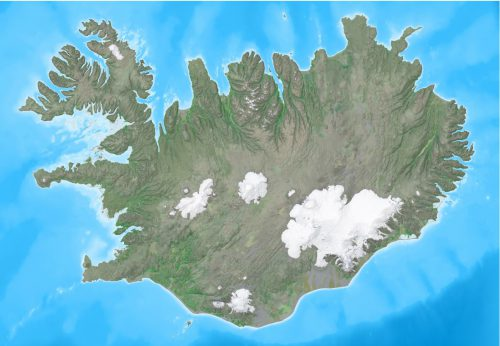
\includegraphics[width=0.21\textwidth, clip, trim=0 0 0 1mm]{Map}};
            \node[anchor=north] (photo) at ($(plan.south west)!0.5!(sectionTitle.south west |- plan.south)-(0,1mm)$) {
                \ifCompileWithPhotos%
                    \IfImageCanBeIncluded{#2}{%
                        \includegraphics[width=0.85\textwidth]{#2}
                    }{%
                        \includegraphics[width=0.75\textwidth]{example-image-a}
                    }
                \else
                    \includegraphics[width=0.75\textwidth]{example-image-a}
                \fi
            };
            \node[text depth=0.5ex, below = 2mm of photo.south east, anchor=north east, xshift=-2pt]{#3};
            \ifthenelse{\isempty{#1}}{}%
            {
                \begin{scope}[x={($ (plan.south east) - (plan.south west) $ )},y={( $ (plan.north west) - (plan.south west)$ )}, shift={(plan.south west)}]
                    %\draw[help lines,xstep=.1,ystep=.1] (0,0) grid (1,1);
                    \node[anchor=south, inner sep=0] at (#1) {
\includegraphics[width=2mm]{Pin}};
                \end{scope}
            }
            \ifCompileWithPhotos
                \IfImageCanBeIncluded{#2}{%
                    \node[rotate=90, anchor=west, font=\ssmall] at ($(current page.south east)+(-2mm,1mm)$) {{\raisebox{-2mm}{\Large\textcopyright}} Photo: All rights are reserved};
                }{}
            \fi
        \end{tikzpicture}
    }
    %Add a link to table of content on frames with a footline
    \addtobeamertemplate{footline}{}{%
        \ifAddLinkToTOC%
            \begin{tikzpicture}[remember picture,overlay]
                %xelatex needs \XeTeXLinkBox, won't create a link unless it
                %finds text --- rules don't work without \XeTeXLinkBox.
                %Still builds correctly with pdflatex and lualatex
                \node[anchor=south east, inner sep=2pt] at (current page.south east) {\hyperlink{toc}{\XeTeXLinkBox{
\includegraphics[width=3mm]{TOC}}}};
            \end{tikzpicture}%
        \fi%
    }%
}

\makeatletter
\AtBeginSection[]% <- Empty optional argument, do nothing for \section*
{%
    \ifnum\beamer@tocsectionnumber>0%
        \begin{frame}[plain, noframenumbering]{}
             \sectionpage
        \end{frame}
    \fi
}
\makeatother

%Append code to put third CSC logo on titlepage
\appto\titlepage{%
    \begin{tikzpicture}[remember picture, overlay]
        \node[anchor=south] at (current page.south) {
\includegraphics[width=25mm]{LogoCSC}};
    \end{tikzpicture}
}

%===============================================================%
\title{Introduction to Bash scripting language}
\author{Alessandro Sciarra \texorpdfstring{\\}{} {\tiny Z02~--~Software Development Center}}
\institute{Organised by the CSC Frankfurt}
\titlegraphic{
\includegraphics[width=20mm]{LogoCRC}}
\titlepagelogo{
\includegraphics[width=20mm]{LogoGoethe}}
%===============================================================%


%===================%
\subtitle{Day 1}
\date{07.10.2019}
%===================%

\begin{document}
    %-------------------------------%
%  Author: Alessandro Sciarra   %
%    Date: 5 Jun 2019           %
%-------------------------------%

%~~~~~~~~~~~~~~~~~~~~~~~~~~~~~~~~~~~~~~~~~~~~%
\begin{frame}[plain,noframenumbering]
    \titlepage
\end{frame}
%~~~~~~~~~~~~~~~~~~~~~~~~~~~~~~~~~~~~~~~~~~~~%
\begin{frame}[plain,noframenumbering]{Topics of the day}
    \medskip
    \begin{columns}[t]
        \begin{column}{.45\textwidth}
            \hspace*{4mm}
            \begin{minipage}[t][0.6\textheight]{\textwidth}
                \tableofcontents[sections={1-6}]
            \end{minipage}
        \end{column}
        \begin{column}{.45\textwidth}
            \begin{minipage}[t][0.6\textheight]{\textwidth}
                \tableofcontents[sections={7-}]
            \end{minipage}
        \end{column}
    \end{columns}
\end{frame}
%~~~~~~~~~~~~~~~~~~~~~~~~~~~~~~~~~~~~~~~~~~~~%

    \addSection{Inception and Philosophy}{example-image-a}{distribution image}
    %-------------------------------%
%  Author: Alessandro Sciarra   %
%    Date: 21 Sep 2020          %
%-------------------------------%

%~~~~~~~~~~~~~~~~~~~~~~~~~~~~~~~~~~~~~~~~~~~~%
\begin{frame}{An often mistreated language}
    \begin{itemize}
        \item Everybody uses Bash
        \item It is easy to know a bit of many commands\tikzmark{arrowfrom}
        \item Not so many Bash users (have time to) go deeply into the details
    \end{itemize}
    \begin{varblock}{alerted}[0.8\textwidth]{The nature of Bash}
        \PQ{As with many tools, it is common to just get stuff working, no matter how}
    \end{varblock}
    %\vspace{2mm}
    \begin{overlayarea}{\textwidth}{0.6\textheight}
        \begin{varblock*}{example}[0.8\textwidth]{Important aspects to \textbf{always} keep in mind}<only@2>
            $\circ\;$Use a clear, readable layout\\
            $\circ\;$Avoid unnecessary commands\\
            $\circ\;$A small, trivial script today might become large and complex tomorrow
        \end{varblock*}
        \begin{tikzpicture}[remember picture, overlay]
            \path[to, PT] (arrowfrom) ++(5mm,0) edge[out=20, in=60, looseness=3]  ++(22mm, -11mm) coordinate (arrival);
            \path[to, visible on=<2>, PS] (arrival)   ++(-53mm,-18mm) edge[out=200, in=150, looseness=2] ++(0mm, -13mm);
        \end{tikzpicture}
        \begin{varblock}{quote}[0.9\textwidth]{Before you get too excited}[Greg's Wiki]<only@3>
            It is key that you remember, Bash is a tool, a single tool in a huge toolbox of programs.
            Bash alone will only let you do basic things with files and other programs.
            You will need to understand all the other tools in the toolbox of your system.
            This knowledge is vast and will come slowly, it is important that you take the time to learn them well rather than try to get the basic idea of most and break a leg tomorrow (or more likely, your music archive or collection of family pictures).
        \end{varblock}
    \end{overlayarea}
\end{frame}
%~~~~~~~~~~~~~~~~~~~~~~~~~~~~~~~~~~~~~~~~~~~~%
\begin{frame}[fragile]{Using Bash}
    \vspace{-2mm}
    \begin{description}
        \item[Bash in interactive mode:] A prompt and a command line
        \item[Bash in non-interactive mode:] Executing scripts
    \end{description}
    \begin{varblock*}{}[0.7\textwidth]{The prompt}
        \texttt{\PQ{cool-prompt}\PT{\$}} $\;\leftarrow\;$ shell compatible with the Bourne shell\\
        \texttt{\PQ{cool-prompt}\PT{\%}} $\;\leftarrow\;$ C-shell (which is not covered here)\\
        \texttt{\PQ{cool-prompt}\PT{\#}} $\;\leftarrow\;$ shell run as superuser (root)
    \end{varblock*}
    \begin{onlyenv}<2>
        \begin{lstlisting}[style=MyBash, aboveskip=5mm]
            $ man man      # Learn how to use and read the manual@|$^\star$|@
            $ man apropos
            $ help         # Get help for builtin commands
            $ help echo
        \end{lstlisting}
        \medskip
        \hfill {\scriptsize $^\star\;$Use \keystroke{Q} to quit the manual}\hspace{1cm}
    \end{onlyenv}
    \begin{varblock*}{example}[0.7\textwidth]{Manual \textbf{SYNOPSIS}}<only@3>
        \footnotesize
        \begin{tabular}{@{\qquad}ll}
            \textbf{bold text}                       &    type exactly as shown.\\
            \underline{italic} \underline{text}      & replace with appropriate argument.\\
            {}[-abc]                                 & any or all arguments within [ ] are optional.\\
            -a|-b                                    & options delimited by | cannot be used together.\\
            \underline{\smash{argument}} ...         & argument is repeatable.\\
            {}[~\underline{\smash{expression}}~] ... & entire expression within [ ] is repeatable.\\
        \end{tabular}
    \end{varblock*}
\end{frame}
%~~~~~~~~~~~~~~~~~~~~~~~~~~~~~~~~~~~~~~~~~~~~%
\begin{frame}{The goal of the day}
    \begin{itemize}
        \item \alert<2>{Arguments}\tikzmark{ptA}
        \item \alert<2>{Quotes}\tikzmark{ptB}
        \item Shell parameters
        \item Special variables (e.g. \bash{IFS})
        \item Shell expansion
              \begin{itemize}
                  \item Brace expansion
                  \item Parameters expansion\tikzmark{ptC}
                  \item \ldots
                  \item \alert<2>{Word splitting}
                  \item Filename expansion
              \end{itemize}
        \item Globbing
        %\item Regular expressions
        %\item Brace expressions
        %\item \bash|if|, \bash|test| and \bash{[[}
    \end{itemize}
    \begin{tikzpicture}[remember picture, overlay, scope on=<2>]
        \coordinate (remark) at ($(ptA)!0.5!(ptC)+(25mm,0)$);
        \node[anchor=west, starburst, minimum height=3cm, starburst point height=8mm, line width=1mm,
              draw=PT, fill=yellow, fill opacity=0.3, text opacity=1, text=PQ,
              visible on=<2>, fill on=<2>, text on=<2>] (cloud) at ($(remark)+(3mm,0)$) {The Bash inner core};
        \node[below = 25mm of cloud, text=PP, rounded corners=3pt, draw=PB, thick, inner sep=2mm] (learn) {Take your time and learn them well!};
        \draw[to, shorter={2mm}{1mm}] (cloud.south) -- (learn);
    \end{tikzpicture}
    \FrameRemark<2>{\PQ{\textbf{Disclaimer:}} \alert{Some slides will unavoidably refer to later material. Hopefully, everything will be clarified at the end of the day and, for sure, by Friday!}}
\end{frame}
%~~~~~~~~~~~~~~~~~~~~~~~~~~~~~~~~~~~~~~~~~~~~%

    \addSection{Commands and arguments}[0.5,0.5]{example-image-b}{image}
    %-------------------------------%
%  Author: Alessandro Sciarra   %
%    Date: 17 Jun 2019          %
%-------------------------------%

%~~~~~~~~~~~~~~~~~~~~~~~~~~~~~~~~~~~~~~~~~~~~%
\begin{frame}[fragile]{How does Bash interpret a line of code?}
    \begin{itemize}
        \item Bash divides each line into words that are demarcated by a \textbf{whitespace character}$^\star$.\tikzmark{whitespace}
        \item \alert{The first word} of the line is the name of \alert{the command} to be executed.
        \item \PP{All the remaining words} become \PP{arguments} to that command (options, filenames, etc.).
    \end{itemize}
    \begin{lstlisting}[style=MyBash, showspaces=true, aboveskip=1mm]
         $@|~|@command arg1 arg2   arg3       arg4
         $@|~|@command arg1 arg2 arg3 arg4
    \end{lstlisting}
    \vspace{2mm}
    \begin{varblock}{alerted}[0.75\textwidth]{}
        \PQ{The amount of whitespace between arguments does not matter!}
    \end{varblock}
    \begin{lstlisting}[style=MyBash, aboveskip=2mm]
        $ echo I am Clark Kent
        |+I am Clark Kent+|                        # <- Same output
        $ echo I    am  Clark         Kent
        |+I am Clark Kent+|                        # <- as here!
    \end{lstlisting}
    \FrameRemark{$^\star$There are a few advanced cases, such as commands that span multiple lines, that have slightly different rules.}
    \begin{tikzpicture}[remember picture, overlay]
        \node[above= 8mm of whitespace, anchor=east, font=\scriptsize, xshift=4pt] (label) {Spaces and Tabs};
        \path[to] (label) edge[out=0, in=0, looseness=1.8] (whitespace);
    \end{tikzpicture}
\end{frame}
%~~~~~~~~~~~~~~~~~~~~~~~~~~~~~~~~~~~~~~~~~~~~%
\begin{frame}[fragile]{The first hurdle: spaces}{How can a so innocent, invisible character hurt me? ...well...}
    \vspace{-3mm}
    \begin{itemize}
        \item To a shell, whitespace is incredibly important
        \item Don't be fooled into thinking a space or tab more or less won't make much of a difference
        \item  Whitespace is \textbf{vital} to allowing your shell to understand you
    \end{itemize}
    \begin{lstlisting}[style=MyBash, aboveskip=4mm]
        $ ls -1
        |+The secret voice.mp3
        secret+|
        $ rm The secret voice.mp3  # rm gets 3 arguments, not 1!
        |+rm: cannot remove 'The': No such file or directory+|
        |+rm: cannot remove 'voice.mp3': No such file or directory+|
        $ ls
        |+The secret voice.mp3+|       # Where's your file 'secret'!?
    \end{lstlisting}
    \centerline{\ssmall \bash|ls| and \bash|rm| are commands to list the present working directory content and to remove files, respectively.}
    \vspace{-3mm}
    \begin{overlayarea}{\textwidth}{0.3\textheight}
        \begin{varblock}{example}[0.5\textwidth]{}<only@1>
            We will deepen into \PS{Word splitting} later!
        \end{varblock}
        \begin{varblock}{}[0.9\textwidth]{Side remark}<only@2>
            \PB{Whitespaces in filenames} should be avoided and \PB{replaced by underscores}. Everything would be much easier. But they are allowed... so deal with it!
        \end{varblock}
    \end{overlayarea}
\end{frame}
%~~~~~~~~~~~~~~~~~~~~~~~~~~~~~~~~~~~~~~~~~~~~%
    \addSection{Strings and type of commands}[0.5,0.5]{example-image-b}{image}
    %-------------------------------%
%  Author: Alessandro Sciarra   %
%    Date: 23 Sep 2020          %
%-------------------------------%

%~~~~~~~~~~~~~~~~~~~~~~~~~~~~~~~~~~~~~~~~~~~~%
\begin{frame}[noframenumbering, plain]{After all it is simple...}
    \centering
    
\includegraphics[width=0.9\textwidth]{ToyStory}
\end{frame}
%~~~~~~~~~~~~~~~~~~~~~~~~~~~~~~~~~~~~~~~~~~~~%
\begin{frame}{Strings, strings everywhere}
    \vspace{-3mm}
    The term string refers to a sequence of characters which is treated as a single unit:
    \begin{itemize}
        \item The command's name is a string
        \item Each argument of a command is a string
        \item Variable names are strings
        \item The contents of variables are strings as well
        \item A filename is a string
        \item Most files contain strings
    \end{itemize}
    \begin{varblock}{alerted}[0.7\textwidth]{Strings do not have any intrinsic meaning}
        Their meaning is defined by how and where they are used. 
    \end{varblock}
    \begin{varblock}{}[0.85\textwidth]{We have \textbf{all} the responsibility}
        We need to be sure everything that needs to be separated is separated properly, and everything that needs to stay together stays together properly!
    \end{varblock}
    \FrameRemark{I will loosely use the term \textbf{string} throughout the lecture, mostly referring to a portion of text contained in a variable}
\end{frame}
%~~~~~~~~~~~~~~~~~~~~~~~~~~~~~~~~~~~~~~~~~~~~%
\begin{frame}<1>[fragile, label=CommandsTypes]{Types of commands}
    \only<1>{\framesubtitle{There are basically 5 different classes of commands}}
    \only<2->{\framesubtitle{}}
    \begin{onlyenv}<1>
        \begin{center}
            \begin{tikzpicture}
                \node[minimum size=5cm, circle, draw, thin] (O) at (0,0) {};
                \foreach \l [count=\li, evaluate=\li as \angle using int(\li*72)] in {Aliases, Functions, Builtins, Keywords, Executables}{
                    \node[cloud, draw, text=PB, fill=PP!20, aspect=2] at (O.\angle) {\l};
                }
            \end{tikzpicture}
        \end{center}
    \end{onlyenv}
    \vspace{-6mm}
    \begin{onlyenv}<2->
        \setlength{\columnsep}{-5mm}
        \begin{multicols}{5}
            \begin{enumerate}
                \item \tc<2>{PP}{Aliases}
                \item \tc<3>{PP}{Functions}
                \item \tc<4-6>{PP}{Builtins}
                \item \tc<7>{PP}{Keywords}
                \item \tc<8>{PP}{Executables}
            \end{enumerate}
        \end{multicols}
    \end{onlyenv}
    \vspace{-3mm}
    \begin{overlayarea}{\textwidth}{0.7\textheight}
        \begin{onlyenv}<2>
            \begin{itemize}
                \item An alias is a rudimentary way of shortening a command
                \item \PP{It is a word that is mapped to a certain string}
                \item They are only used in \textbf{interactive} shells and \textbf{not} in scripts
                \item They are limited in power; the replacement only happens in the first word
                \item An alias should effectively not do more than change the default options of a command
                \item For more complex tasks and more flexibility, use a function
            \end{itemize}
            \begin{lstlisting}[style=MyBash]
                $ help alias
                |+alias: alias [-p] [name[=value] ... ]+|
                |+    Define or display aliases.       +|

                # [More information]

                $ alias ls='ls --color=auto'
                $ ls  # The command executed is, instead:  ls --color=auto
            \end{lstlisting}
            \FrameRemark{Bash stores the values of aliases in an array called \bash|BASH_ALIASES|}
        \end{onlyenv}
        \begin{onlyenv}<3>
            {\Large
            \begin{varblock}{alerted}[0.7\textwidth]{Functions are tricky!}
                They will be covered in depth later in the course
            \end{varblock}}
            \bigskip
            For the moment, a few hints:
            \begin{itemize}
                \item Functions in Bash are more powerful than aliases and the are often the way to go
                \item Unlike aliases, they can be used in scripts, i.e. in non-interactive mode
                \item A function contains shell commands, and acts very much like a small script
                \item They can even take arguments and create local variables
                \item When a function is called, the commands in it are executed
            \end{itemize}
        \end{onlyenv}
        \begin{onlyenv}<4-6>
            \begin{itemize}
                \item Builtins are basic commands that Bash has built into it
                \item They can be thought as functions that are already provided
                \item We will learn about (or at least mention) \tc<5>{PP}{most of them}
                \item Keywords which are provided as builtins are nevertheless highlighted as \tc<6>{keywords-color}{keywords}
            \end{itemize}
            \begin{onlyenv}<4>
                \begin{lstlisting}[style=MyBash, numbers=none, keywordstyle=\color{builtins-color},]
                   :         complete   export    let        shift     umask  
                   .         compgen    false     local      shopt     unalias
                   [         continue   fc        logout     source    unset  
                   alias     declare    fg        popd       suspend   until  
                   bg        dirs       getopts   printf     test      wait   
                   bind      disown     hash      pushd      times     while  
                   break     echo       help      pwd        trap      
                   builtin   enable     history   read       true      
                   case      eval       if        readonly   type      
                   cd        exec       jobs      return     typeset   
                   command   exit       kill      set        ulimit    
                \end{lstlisting}
            \end{onlyenv}
            \begin{onlyenv}<5>
                \begin{lstlisting}[style=MyBash, numbers=none, deleteemph={[5]:,.,[,alias, bg, bind, break, case, cd, complete, compgen, continue, declare, dirs, disown, echo, eval, exec, exit, export,false, fg, help, if, jobs, kill, let, local, popd, printf, pushd, pwd, read, readonly, return, set, shift, shopt, source, test, trap, true, unalias, unset, until, wait, while}, emph={[7]:,.,[,alias, bg, bind, break, case, cd, complete, compgen, continue, declare, dirs, disown, echo, eval, exec, exit, export,false, fg, help, if, jobs, kill, let, local, popd, printf, pushd, pwd, read, readonly, return, set, shift, shopt, source, test, trap, true, unalias, unset, until, wait, while}, emphstyle={[7]\color{PP}}]
                   :         complete   export    let        shift     umask  
                   .         compgen    false     local      shopt     unalias
                   [         continue   fc        logout     source    unset  
                   alias     declare    fg        popd       suspend   until  
                   bg        dirs       getopts   printf     test      wait   
                   bind      disown     hash      pushd      times     while  
                   break     echo       help      pwd        trap      
                   builtin   enable     history   read       true      
                   case      eval       if        readonly   type      
                   cd        exec       jobs      return     typeset   
                   command   exit       kill      set        ulimit    
                \end{lstlisting}
            \end{onlyenv}
            \begin{onlyenv}<6>
                \begin{lstlisting}[style=MyBash, numbers=none]
                   :         complete   export    let        shift     umask  
                   .         compgen    false     local      shopt     unalias
                   [         continue   fc        logout     source    unset  
                   alias     declare    fg        popd       suspend   until  
                   bg        dirs       getopts   printf     test      wait   
                   bind      disown     hash      pushd      times     while  
                   break     echo       help      pwd        trap      
                   builtin   enable     history   read       true      
                   case      eval       if        readonly   type      
                   cd        exec       jobs      return     typeset   
                   command   exit       kill      set        ulimit    
                \end{lstlisting}
            \end{onlyenv}
        \end{onlyenv}
        \begin{onlyenv}<7>
            \begin{varblock}{alerted}[0.75\textwidth]{}
                Keywords are like builtins, but \alert{special parsing rules apply to them}
            \end{varblock}
            \begin{itemize}
                \item Flow control constructs is achieved thanks to keywords
                \item We will explore all of them in detail \Remark[2mm]{except \bash|coproc|}
            \end{itemize}
            \begin{lstlisting}[style=MyBash, numbers=none]
                if     elif   esac     while   done      time   !    coproc
                then   fi     for      until   in        {      [[
                else   case   select   do      function  }      ]]
            \end{lstlisting}
            \bigskip
            For example:
            \medskip
            \begin{lstlisting}[style=MyBash]
                $ [ a < b ]   # Oops, < means here input redirection!
                |+-bash: b: No such file or directory+|
                $ [[ a < b ]] # The meaning of < changes within [[ ]]
            \end{lstlisting}
        \end{onlyenv}
        \begin{onlyenv}<8>
            \begin{itemize}
                \item Executables are the last type of command that Bash can execute
                \item They are also known as external commands or applications
                \item They are typically invoked by their name, on the constraint that Bash is able to find them
                \item When a command is specified without a file path and it is \alert{not an alias, a function, a builtin or a keyword}, Bash searches through the directories contained in the variable \bash|PATH|
                \item The search is done from left to right and the first executable found is run
            \end{itemize}
            \begin{lstlisting}[style=MyBash]
                $ ls /home/sciarra/.local/bin
                |+...   g++   ...+| # Version 8.3.0
                $ ls /usr/bin
                |+...   g++   ...+| # Version 5.4.0
                $ echo ${PATH}
                |+/home/sciarra/.local/bin:/usr/bin:/bin+|
                $ g++ -dumpversion
                |+8.3.0+|
            \end{lstlisting}
        \end{onlyenv}
    \end{overlayarea}
\end{frame}
%~~~~~~~~~~~~~~~~~~~~~~~~~~~~~~~~~~~~~~~~~~~~%
\againframe<2>{CommandsTypes}
%~~~~~~~~~~~~~~~~~~~~~~~~~~~~~~~~~~~~~~~~~~~~%
\againframe<3>{CommandsTypes}
%~~~~~~~~~~~~~~~~~~~~~~~~~~~~~~~~~~~~~~~~~~~~%
\againframe<4-6>{CommandsTypes}
%~~~~~~~~~~~~~~~~~~~~~~~~~~~~~~~~~~~~~~~~~~~~%
\againframe<7>{CommandsTypes}
%~~~~~~~~~~~~~~~~~~~~~~~~~~~~~~~~~~~~~~~~~~~~%
\againframe<8>{CommandsTypes}
%~~~~~~~~~~~~~~~~~~~~~~~~~~~~~~~~~~~~~~~~~~~~%
\begin{frame}[fragile]{Bash scripts}
    \vspace{-6mm}
    \begin{itemize}
        \item A script is a sequence of Bash commands in a file
        \item The commands are read and processed \PP{in order}
        \item A new command is processed after the previous has \PP{ended} \Remark{unless differently required}
        \item The first line of a script should be reserved for an \textbf{interpret directive} also called \alert{hashbang} or \alert{shebang}.
              This is used when the kernel executes a non-binary file.
              Use one of the two following alternatives: \\
              \begin{center}
                  \begin{tikzpicture}
                      \node[fill=background-color, inner sep=1mm, font=\scriptsize] (shebangA) {\bash|#!/bin/bash|};
                      \node[fill=background-color, inner sep=1mm, font=\scriptsize, right = 3cm of shebangA] (shebangB) {\bash|#!/usr/bin/env bash|};
                      \draw[to, shorter={2mm}{2mm}] (shebangA) -- node[midway, above=-1pt, font=\tiny] {or, preferably,} (shebangB);
                  \end{tikzpicture}
                  \par{\ssmall The right directive has the benefit of looking for whatever the default version of the program is in your current \textbf{env}ironment (i.e. in \bash|PATH|).}
              \end{center}
        \item<only@1> Please, \alert{do not use} \,\raisebox{0.1em}{\fbox{\ssmall\bash|#!/bin/sh|}}\, as shebang, even if you might see it around on the web!
        \item<only@1> Avoid giving your scripts a \textbf{.sh} extension. Do not use one or use \alert{\textbf{.bash}}!
        \item<only@2> Execute the script in either of the following ways:
    \end{itemize}
    \begin{varblock}{alerted}[0.75\textwidth]{\textbf{Sh is NOT Bash!}}<only@1>
        \textbf{Bash} itself is a \textbf{sh-compatible} shell however, the opposite is not true!
    \end{varblock}
    \begin{onlyenv}<2>
        \begin{lstlisting}[style=MyBash]
            $ bash myscript   #The shebang is treated as a comment!
        \end{lstlisting}
        \centerline{or}
        \begin{lstlisting}[style=MyBash]
            $ chmod +x myscript  # Make the file executable
            $ ./myscript         # Execute it, the shebang is used!
        \end{lstlisting}
    \end{onlyenv}
\end{frame}
%~~~~~~~~~~~~~~~~~~~~~~~~~~~~~~~~~~~~~~~~~~~~%



    \addSection{Quoting and Special characters}[0.5,0.5]{example-image-b}{image}
%     \input{Slides/}
    \addSection{Parameters (a.k.a. Variables)}[0.5,0.5]{example-image-b}{image}
%     \input{Slides/}
    \addSection{Special variables}[0.5,0.5]{example-image-b}{image}
%     \input{Slides/}
    \addSection{Parameter Expansion}[0.5,0.5]{example-image-b}{image}
%     \input{Slides/}
    \addSection{Word splitting}[0.5,0.5]{example-image-b}{image}
%     \input{Slides/}
    \addSection{Command line arguments}[0.5,0.5]{example-image-b}{image}
%     \input{Slides/}
    \addSection{Patterns}[0.5,0.5]{example-image-b}{image}
%     \input{Slides/}
    \addSection{Conditionals and tests}[0.5,0.5]{example-image-b}{image}
%     \input{Slides/}
    \addSection{Road to the exercises}[0.5,0.5]{example-image-b}{image}
\end{document}
